\documentclass{article}

\usepackage[final]{neurips_2019}

\usepackage[utf8]{inputenc}
\usepackage[T1]{fontenc}
\usepackage{url}
\usepackage{booktabs}
\usepackage{amsfonts}
\usepackage{amssymb}
\usepackage{nicefrac}
\usepackage{microtype}
\usepackage{graphicx}
\usepackage{verbatim}
\usepackage{xcolor}
\usepackage{lipsum}
\usepackage{xcolor}
\usepackage[colorlinks = true,
            linkcolor = blue,
            urlcolor  = blue,
            citecolor = blue,
            anchorcolor = blue]{hyperref}
\newcommand{\note}[1]{\textcolor{blue}{{#1}}}
\newcommand{\abs}[1]{\left| #1\right|}
\usepackage{amsmath}

\title{
  Translating Natural Language to Bash Commands using Deep Neural Networks \\
  \vspace{1em}
  \small{\normalfont Stanford CS224N Custom Project}
}

\author{
 Daniel Jenson \\
  Department of Management Science \& Engineering \\
  Stanford University \\
  \texttt{djenson@stanford.edu} \\
  % Examples of more authors
  \And
  Yingxiao Liu \\
  Department of Civil and Environmental Engineering \\
  Stanford University \\
  \texttt{liuyx@stanford.edu} \\
}

\begin{document}

\maketitle

\begin{abstract}
	The objective of this project is to generate bash commands from natural
	language using a deep neural network. We are experimenting with several models,
	including GPT-2, BART, and T5, as well as different tokenization schemes to
	improve model performance on the NLC2CMD dataset. We have successfully
	trained a GPT-2 model, which has achieved modest performance. Next, we will
	next train models using BART and T-5. However, we suspect that the majority
	of gains may be achieved from improved encoding and tokenization.
\end{abstract}


\section{Key Information to include}
\begin{itemize}
	\item TA mentor: Ethan A. Chi
	\item External collaborators: No
	\item External mentor: No
	\item Sharing project: No
\end{itemize}

% {\color{red} This template does not contain the full instruction set for this assignment; please refer back to the milestone instructions PDF.}

\section{Introduction}
The objective of this project is to generate bash commands from natural
language using a deep neural network. Novitiates often find the terminal
interface perplexing and are quickly overwhelmed by the syntax of bash
commands. Even experienced engineers frequently consult man-pages, online
documentation, and online forums like StackOverflow to learn about the
particulars of various commands. This project aims to ease that burden on new
and experienced users alike. An interesting minimum viable product in this
space in this space is ``aish,'' short for AI-shell, which is part of the
\href{http://anix.org}{AInix} Kernel project. In the future, we hope that this
field of research will be able to construct sequences of bash commands,
automating entire workflows from simple natural language descriptions. However,
for this project, we focus solely on executing atomic commands.
% TODO: Yinxaio, clean up and embellish
% The introduction explains the problem, why it's difficult, interesting, or important, how and why current methods succeed/fail at the problem, and explains the key ideas of your approach and results. Though an introduction covers similar material as an abstract, the introduction gives more space for motivation, detail, references to existing work, and to capture the reader's interest.

\section{Related Work}
This section helps the reader understand the research context of your work, by providing an overview of existing work in the area.
% TODO: Yingxiao summarize preview work, maybe add a second article -- the one that won the competition

\color{red}
\section{Approach}
\color{black}
The NLC2CMD Challenge was held once by NeurIPS in 2020. The provided dataset
consists of 10,000 parallel translations as a JSON. The goal for competitors
was to generate templated commands from natural language commands that could be
used to guide bash users. Most competitors used GPT2 as their base model. This
paper also uses GPT2 but also surveys two additional models, BART and T5,
version 1.1.
\par
The general approach consisted of two principle methods: (1) text generation
and (2) translation. First, it is important to note that Bash is not a
context-free grammar. It admits of very little recursion and, while most
binaries are POSIX compliant, their interfaces are non-standardized. Flags
often carry different semantic meaning and imply different tasks when employed
by different binaries. Moreover, flags often override, modify, or cancel the
intent of other flags in the same command, introducing complex dependencies.
These dependencies can also shift as the order of the flags and their arguments
are permuted. In sum, the meaning of a flag is almost entirely provided by the
invoking binary and its location in the sequence of arguments. This introduces
difficulties in fine-tuning embeddings, since training may attempt to encode
vastly different meanings in the same embedding. This is particularly
challenging given sparse datasets. Given sufficient training data, it is likely
that that the models may eventually learn correct contextual meaning when
employed by different binaries, but we found 10,000 rows insufficient for the
task. This line of thinking inspired our first approach, text generation using
GPT2.
\par
While at first this task appears to be a straightforward translation task,
after considering bash more closely, one can see that it does not admit of many
properties or structures of natural language. Accordingly, we thought that
rather than trying to properly translate natural language into bash, we could
train a model to hallucinate bash ``stories'' given natural language. The
high-level idea here is that we fine-tune a GPT2 model, showing it complete
stories that consist of both a natural language portion and a bash portion with
some added special tokens. When training, GPT2 learns common storylines,
and when testing, we feed the trained model only the first half of the
story, i.e. the natural language portion, and ask it to complete the story,
hoping that it will generate bash commands as the most likely story completion.
In many respects, this idea performs quite well; however, a significant issue
with this approach is constraining responses from GPT2. How long should the
story be? When does the real content of the ``bash story'' start and end? What
happens when GPT2 has multiple endings? These questions are detailed in the
error analysis section.
\par
The second approach we used was a more traditional seq2seq language modeling
approach. Pre-trained models for BART and T5 are easily fine-tuned for
translation tasks. While many natural language modeling tasks admit of a fair
amount of transfer learning because natural languages share some abstract
semantic structures, bash does not benefit from this nearly as much. As a
non-natural, non-context-free grammar language, modeling it can be difficult,
and our BART model, in particular, struggled with this.

\section{Experiments}
\subsection{Data}
Describe the dataset(s) you are using (provide references). If it's not already clear, make sure the associated task is clearly described.
Being precise about the exact form of the input and output can be very useful for readers attempting to understand your work, especially if you've defined your own task.
% TODO: review templating / AST
% TODO: show tokenization examples
% The competition also provided several utilities of which we availed ourselves.
% First, they released a bash to AST parser, which can also write an AST back to
% a templated form, e.g. replacing file paths with ``File'' and regular
% expressions with the token ``Regex.'' This allows the model to learn
% placeholder values for commands. They also provided a function to compute their
% competition scoring metric, which we use to establish our baseline.

\subsection{Evaluation method}
% TODO: Yingxiao clean up
The competition clearly defined a metric for evaluation, which we used. The
data consists of natural language to bash command pairs. Our model, $A$,
will implement a top 5 translator from a natural language command, $nlc$, to a
prediction, $c$, and confidence, $\delta$, tuple.
\[
	\begin{aligned}
		G(nlc)
		 & =\{C\mid \text{Bash command that achieves the task described in} nlc\} \\
		A : nlc
		 & \rightarrow \{p \mid p = \langle c, \delta\rangle\}                    \\
		|A(nlc)|
		 & \le 5                                                                  \\
	\end{aligned}
\]
The normalized score of a prediction, $p=\langle c, \delta\rangle$ is:
\[
	\begin{aligned}
		S(p)
		 & = \max_{C\in G(nlc)}\sum_{i\in[1,T]}\frac{\delta}{T}\times\left(
		\mathbb{I}[U(c)_i=U(C)i]\times\frac{1}{2}\left(
			1+\frac{1}{N}\left(X\right)\right) -\mathbb{I}[U(c)_i\ne U(C)_i]
		\right)                                                                    \\
		\text{where}
		 &                                                                         \\
		X
		 & = 2\times \abs{F(U(c)_i)\cap F(U(C)_i)} - \abs{F(U(c)_i)\cup F(U(C)_i)} \\
		U(c)
		 & = \text{sequence of Bash utilities in a command $c$}                    \\
		F(u)
		 & = \text{the set of flags for an utility $u$}                            \\
		T
		 & = \max\left(\abs{U(c)}, \abs{U(C)}\right)                               \\
		N
		 & = \max\left(\abs{F(U(c)_i)}, \abs{F(U(C)_i)}\right)                     \\
	\end{aligned}
\]
The overall score is given by the following:
\[
	\begin{aligned}
		Score(A(nlc))
		 & =
		\begin{cases}
			\max_{p\in A(nlc)}S(p),
			 & \text{ if }\exists_{p\in A(nlc)}\text{ such that }S(p) > 0 \\
			\frac{1}{\abs{A(nlc)}}\sum_{p\in A(nlc)}S(p),
			 & \text{otherwise}                                           \\
		\end{cases}
	\end{aligned}
\]
This scoring mechanism promotes precision and recall of the correct binary and
flags, weighted by confidence. There are more caveats and details under the
Task section of the challenge website.
Describe the evaluation metric(s) you use, plus any other details necessary to understand your evaluation.
Some projects will have clear metrics from prior work on given datasets, but we realize that other projects will define their own metrics.
If you're defining your own metrics, be clear as to what you're hoping to measure with each evaluation method (whether quantitative or qualitative, automatic or human-defined!), and how it's defined.

\color{red}
\subsection{Experimental details}
\color{black}
For this task, we tested 3 models: HuggingFace's
\href{https://huggingface.co/gpt2}{GPT2}\cite{gpt2},
\href{https://huggingface.co/facebook/bart-large}{Facebook's BART
	Large}\cite{bart}, and \href{https://huggingface.co/google/t5-v1_1-base}{Google's T5 v1.1
	base}. GPT2 was a causal model, predicting text from context, while the other
two were traditional seq2seq models. Each was trained for 5, 10, and 25
epochs. Batch size was limited to 10 examples, except for T5, which had to be
reduced to 5. For training, we used the AdamW optimizer with weight decay
regularization. The learning rate was linear with a warmup of 100 steps. The
dataset was split into 98\% training and 2\% test sets. Given that the
dataset was approximately 10,000 parallel translations, the test set was
slightly over 200 examples. Training time for GPT, BART, and T5v1.1 was
approximately 1, 1.5, and 1.25 hours, respectively, on an Azure NC6 instance
with a Tesla V100 PCIe 16GB GPU. We attemtped training the original T5 large
model, but even with 5 examples per batch, we got out of memory errors, and
it took approximately 6 hours to finetune. All 3 models used cross-entropy
loss for training, but were scored on the test set using the NLC2CMD metric
at the end of each epoch.

\color{red}
\subsection{Results}
\color{black}
% TODO: finish by 2:30 PM

\begin{center}
	\includegraphics[scale=0.4]{loss.png}
	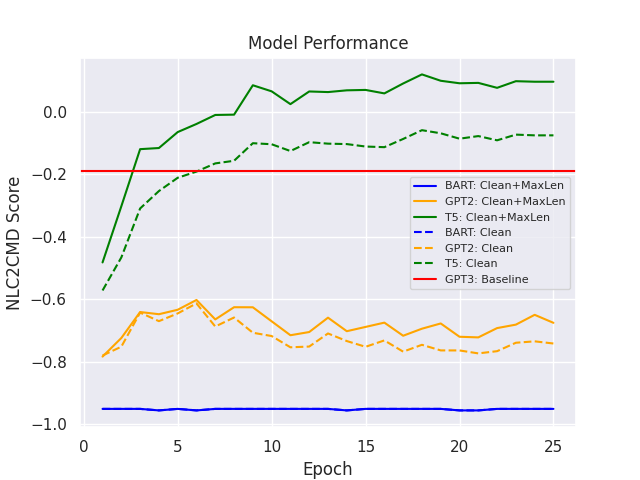
\includegraphics[scale=0.4]{metric.png}
\end{center}
The requirement from the course website: Report the quantitative results that you have found so far. Use a table or plot to compare results and compare against baselines.
Comment on your quantitative results. Are they what you expected? Better than you expected? Worse than you expected? Why do you think that is? What does that tell you about your approach?

Yingxiao's thought: show them the loss-epoch curve, the metric-epoch curve, and one table summarizing the best scores for the gpt2, bart, t5, and baseline gpt3, with different postprocessing functions. Please comment as much as you could in this section. Mention that our results became better and better after more epochs, although the score did not improve. Any thought on the causual / seq2seq models?


\section{Analysis}
Your report should include \textit{qualitative evaluation}. That is, try to understand your system (e.g. how it works, when it succeeds and when it fails) by inspecting key characteristics or outputs of your model.

Dan's thought: include error analysis, why cross-entropy was different from metric, etc.

\section{Conclusion}
Summarize the main findings of your project, and what you have learnt. Highlight your achievements, and note the primary limitations of your work. If you like, you can describe avenues for future work.


\bibliographystyle{unsrt}
\bibliography{references}


\appendix

\section{Appendix (optional)}
If you wish, you can include an appendix, which should be part of the main PDF, and does not count towards the 6-8 page limit.
Appendices can be useful to supply extra details, examples, figures, results, visualizations, etc., that you couldn't fit into the main paper. However, your grader \textit{does not} have to read your appendix, and you should assume that you will be graded based on the content of the main part of your paper only.

\end{document}
